%% LyX 2.1.4 created this file.  For more info, see http://www.lyx.org/.
%% Do not edit unless you really know what you are doing.
\documentclass[twocolumn,english,spanish,journal]{IEEEtran}
\usepackage{newtxmath}
\usepackage[T1]{fontenc}
\usepackage[utf8]{inputenc}
\synctex=-1
\usepackage{babel}
\addto\shorthandsspanish{\spanishdeactivate{~<>}}

\usepackage{float}
\usepackage{booktabs}
\usepackage{calc}
\usepackage[unicode=true,pdfusetitle,
 bookmarks=true,bookmarksnumbered=false,bookmarksopen=false,
 breaklinks=false,pdfborder={0 0 1},backref=false,colorlinks=false]
 {hyperref}

\makeatletter

%%%%%%%%%%%%%%%%%%%%%%%%%%%%%% LyX specific LaTeX commands.
%% Because html converters don't know tabularnewline
\providecommand{\tabularnewline}{\\}
\floatstyle{ruled}
\newfloat{algorithm}{tbp}{loa}
\providecommand{\algorithmname}{Algoritmo}
\floatname{algorithm}{\protect\algorithmname}

%%%%%%%%%%%%%%%%%%%%%%%%%%%%%% Textclass specific LaTeX commands.
 % protect \markboth against an old bug reintroduced in babel >= 3.8g
 \let\oldforeign@language\foreign@language
 \DeclareRobustCommand{\foreign@language}[1]{%
   \lowercase{\oldforeign@language{#1}}}

%%%%%%%%%%%%%%%%%%%%%%%%%%%%%% User specified LaTeX commands.
\usepackage{graphicx}
\usepackage{pgfplots}
\usepgfplotslibrary{groupplots}
\pgfkeys{/pgf/number format/.cd, set thousands separator=\,}

\makeatother

\usepackage{listings}
\addto\captionsenglish{\renewcommand{\algorithmname}{Algorithm}}
\addto\captionsenglish{\renewcommand{\lstlistingname}{Listing}}
\addto\captionsspanish{\renewcommand{\algorithmname}{Algoritmo}}
\addto\captionsspanish{\renewcommand{\lstlistingname}{Listado de código}}
\renewcommand{\lstlistingname}{Listado de código}

\begin{document}

\title{Título del reporte}


\author{Mi nombre y carné}

\selectlanguage{english}%

\markboth{Estructuras de Datos y Análisis de Algoritmos -- Tarea I -- Mi nombre}{}
\maketitle
\selectlanguage{spanish}%
\begin{abstract}
En este trabajo\ldots{} Para esto\ldots{} El resultado fue\ldots{}
Se concluye que\ldots{} (todo en un párrafo).
\end{abstract}


\section{Introducción}

\IEEEPARstart{E}{n este trabajo} se\ldots{} Lorem ipsum dolor sit
amet, consetetur sadipscing elitr, sed diam nonumy eirmod tempor invidunt
ut labore et dolore magna aliquyam erat, sed diam voluptua. At vero
eos et accusam et justo duo dolores et ea rebum. Stet clita kasd gubergren,
no sea takimata sanctus est Lorem ipsum dolor sit amet. Lorem ipsum
dolor sit amet, consetetur sadipscing elitr, sed diam nonumy eirmod
tempor invidunt ut labore et dolore magna aliquyam erat, sed diam
voluptua.

Lorem ipsum dolor sit amet, consetetur sadipscing elitr, sed diam
nonumy eirmod tempor invidunt ut labore et dolore magna aliquyam erat,
sed diam voluptua. At vero eos et accusam et justo duo dolores et
ea rebum. Stet clita kasd gubergren, no sea takimata sanctus est Lorem
ipsum dolor sit amet. Lorem ipsum dolor sit amet, consetetur sadipscing
elitr, sed diam nonumy eirmod tempor invidunt ut labore et dolore
magna aliquyam erat, sed diam voluptua.


\section{Metodología}

Para lograr lo propuesto\ldots{} Lorem ipsum dolor sit amet, consetetur
sadipscing elitr, sed diam nonumy eirmod tempor invidunt ut labore
et dolore magna aliquyam erat, sed diam voluptua. At vero eos et accusam
et justo duo dolores et ea rebum. Stet clita kasd gubergren, no sea
takimata sanctus est Lorem ipsum dolor sit amet. Lorem ipsum dolor
sit amet, consetetur sadipscing elitr, sed diam nonumy eirmod tempor
invidunt ut labore et dolore magna aliquyam erat, sed diam voluptua.

El código se muestra en los apéndices. Este código está basado en
el pseudocódigo del libro de Cormen y colaboradores~\cite{Cormen:2009}.
Lorem ipsum dolor sit amet, consetetur sadipscing elitr, sed diam
nonumy eirmod tempor invidunt ut labore et dolore magna aliquyam erat,
sed diam voluptua. At vero eos et accusam et justo duo dolores et
ea rebum. Stet clita kasd gubergren, no sea takimata sanctus est Lorem
ipsum dolor sit amet. Lorem ipsum dolor sit amet, consetetur sadipscing
elitr, sed diam nonumy eirmod tempor invidunt ut labore et dolore
magna aliquyam erat, sed diam voluptua.

Lorem ipsum dolor sit amet, consetetur sadipscing elitr, sed diam
nonumy eirmod tempor invidunt ut labore et dolore magna aliquyam erat,
sed diam voluptua. At vero eos et accusam et justo duo dolores et
ea rebum. Stet clita kasd gubergren, no sea takimata sanctus est Lorem
ipsum dolor sit amet. Lorem ipsum dolor sit amet, consetetur sadipscing
elitr, sed diam nonumy eirmod tempor invidunt ut labore et dolore
magna aliquyam erat, sed diam voluptua.

Lorem ipsum dolor sit amet, consetetur sadipscing elitr, sed diam
nonumy eirmod tempor invidunt ut labore et dolore magna aliquyam erat,
sed diam voluptua. At vero eos et accusam et justo duo dolores et
ea rebum. Stet clita kasd gubergren, no sea takimata sanctus est Lorem
ipsum dolor sit amet. Lorem ipsum dolor sit amet, consetetur sadipscing
elitr, sed diam nonumy eirmod tempor invidunt ut labore et dolore
magna aliquyam erat, sed diam voluptua.


\section{Resultados}

Los tiempos de ejecución de las X corridas de los algoritmos se muestran
en el cuadro~\ref{tab:tiempos}.
\begin{table}
\caption{Tiempo de ejecución de los algoritmos.\label{tab:tiempos}}


\centering{}%
\begin{tabular}{lrrrrrrr}
\toprule 
 &  & \multicolumn{6}{c}{Tiempo (ms)}\tabularnewline
\cmidrule{3-8} 
 &  & \multicolumn{5}{c}{Corrida} & \tabularnewline
\cmidrule{3-7} 
Algoritmo & Tam. (k) & 1 & 2 & 3 & 4 & 5 & Prom.\tabularnewline
\midrule 
Selección & $10$ & $12.3$ & $12.3$ & $12.3$ & $12.3$ & $12.3$ & $12.3$\tabularnewline
 & $20$ & $12.3$ & $12.3$ & $12.3$ & $12.3$ & $12.3$ & $12.3$\tabularnewline
 & $30$ & $12.3$ & $12.3$ & $12.3$ & $12.3$ & $12.3$ & $12.3$\tabularnewline
 & $40$ & $12.3$ & $12.3$ & $12.3$ & $12.3$ & $12.3$ & $12.3$\tabularnewline
\midrule
Inserción & $10$ & $12.3$ & $12.3$ & $12.3$ & $12.3$ & $12.3$ & $12.3$\tabularnewline
 & $20$ & $12.3$ & $12.3$ & $12.3$ & $12.3$ & $12.3$ & $12.3$\tabularnewline
 & $30$ & $12.3$ & $12.3$ & $12.3$ & $12.3$ & $12.3$ & $12.3$\tabularnewline
 & $40$ & $12.3$ & $12.3$ & $12.3$ & $12.3$ & $12.3$ & $12.3$\tabularnewline
\midrule
Mezcla & $10$ & $12.3$ & $12.3$ & $12.3$ & $12.3$ & $12.3$ & $12.3$\tabularnewline
 & $20$ & $12.3$ & $12.3$ & $12.3$ & $12.3$ & $12.3$ & $12.3$\tabularnewline
 & $30$ & $12.3$ & $12.3$ & $12.3$ & $12.3$ & $12.3$ & $12.3$\tabularnewline
 & $40$ & $12.3$ & $12.3$ & $12.3$ & $12.3$ & $12.3$ & $12.3$\tabularnewline
\bottomrule
\end{tabular}
\end{table}
 Lorem ipsum dolor sit amet, consetetur sadipscing elitr, sed diam
nonumy eirmod tempor invidunt ut labore et dolore magna aliquyam erat,
sed diam voluptua. At vero eos et accusam et justo duo dolores et
ea rebum. Stet clita kasd gubergren, no sea takimata sanctus est Lorem
ipsum dolor sit amet. Lorem ipsum dolor sit amet, consetetur sadipscing
elitr, sed diam nonumy eirmod tempor invidunt ut labore et dolore
magna aliquyam erat, sed diam voluptua.

Los tiempos promedio se muestran gráficamente en la figura~\ref{fig:lin}.
\begin{figure*}
\begin{centering}
\begin{tikzpicture}
    \begin{axis}[name=plot1,width=0.9\columnwidth,xtick={10,20,...,40},ylabel=Tiempo (ms),title=\textbf{Selección}]
        \addplot coordinates{(10,200) (20,600) (30,800) (40,1200)};
    \end{axis}
    \begin{axis}[name=plot2,at={($(plot1.east)+(0.15\textwidth,0)$)},anchor=west,width=0.9\columnwidth,xtick={10,20,...,40},title=\textbf{Inserción}]
        \addplot coordinates{(10,800) (20,1200) (30,400) (40,800)};
    \end{axis}
    \begin{axis}[name=plot3,at={($(plot1.south)-(0,1.5cm)$)},anchor=north,width=0.9\columnwidth,xtick={10,20,...,40},ylabel=Tiempo (ms),title=\textbf{Mezcla}]
        \addplot coordinates{(10,600) (20,500) (30,100) (40,200)};
    \end{axis}
    \begin{axis}[name=plot4,at={($(plot2.south)-(0,1.5cm)$)},anchor=north,width=0.9\columnwidth,xtick={10,20,...,40},title=\textbf{Montículos}]
        \addplot coordinates{(10,600) (20,100) (30,500) (40,100)};
    \end{axis}
    \begin{axis}[name=plot5,at={($(plot3.south)-(0,1.5cm)$)},anchor=north,width=0.9\columnwidth,ylabel=Tiempo (ms),xlabel=Tamaño del arreglo (miles),title=\textbf{Rápido}]
        \addplot coordinates{(10,300) (20,100) (30,200) (40,500)};
    \end{axis}
% Comente las líneas siguientes con '%' si no implementó ordenamiento por residuos
  \begin{axis}[name=plot6,at={($(plot4.south)-(0,1.5cm)$)},anchor=north,width=0.9\columnwidth,xlabel=Tamaño del arreglo (miles),title=\textbf{Residuos}]
        \addplot coordinates{(10,600) (20,200) (30,400) (40,500)};
    \end{axis}
\end{tikzpicture}
\par\end{centering}

\caption{Tiempos promedio de ejecución de los algoritmos de ordenamiento por
selección, inserción, mezcla, montículos, rápido y residuos.\label{fig:lin}}
\end{figure*}
 La forma de las curvas no fueron las esperadas porque inventé los
números. Lorem ipsum dolor sit amet, consetetur sadipscing elitr,
sed diam nonumy eirmod tempor invidunt ut labore et dolore magna aliquyam
erat, sed diam voluptua. At vero eos et accusam et justo duo dolores
et ea rebum. Stet clita kasd gubergren, no sea takimata sanctus est
Lorem ipsum dolor sit amet. Lorem ipsum dolor sit amet, consetetur
sadipscing elitr, sed diam nonumy eirmod tempor invidunt ut labore
et dolore magna aliquyam erat, sed diam voluptua.

Las curvas se muestran de forma conjunta en la figura~\ref{fig:log}.
\begin{figure*}
\begin{centering}
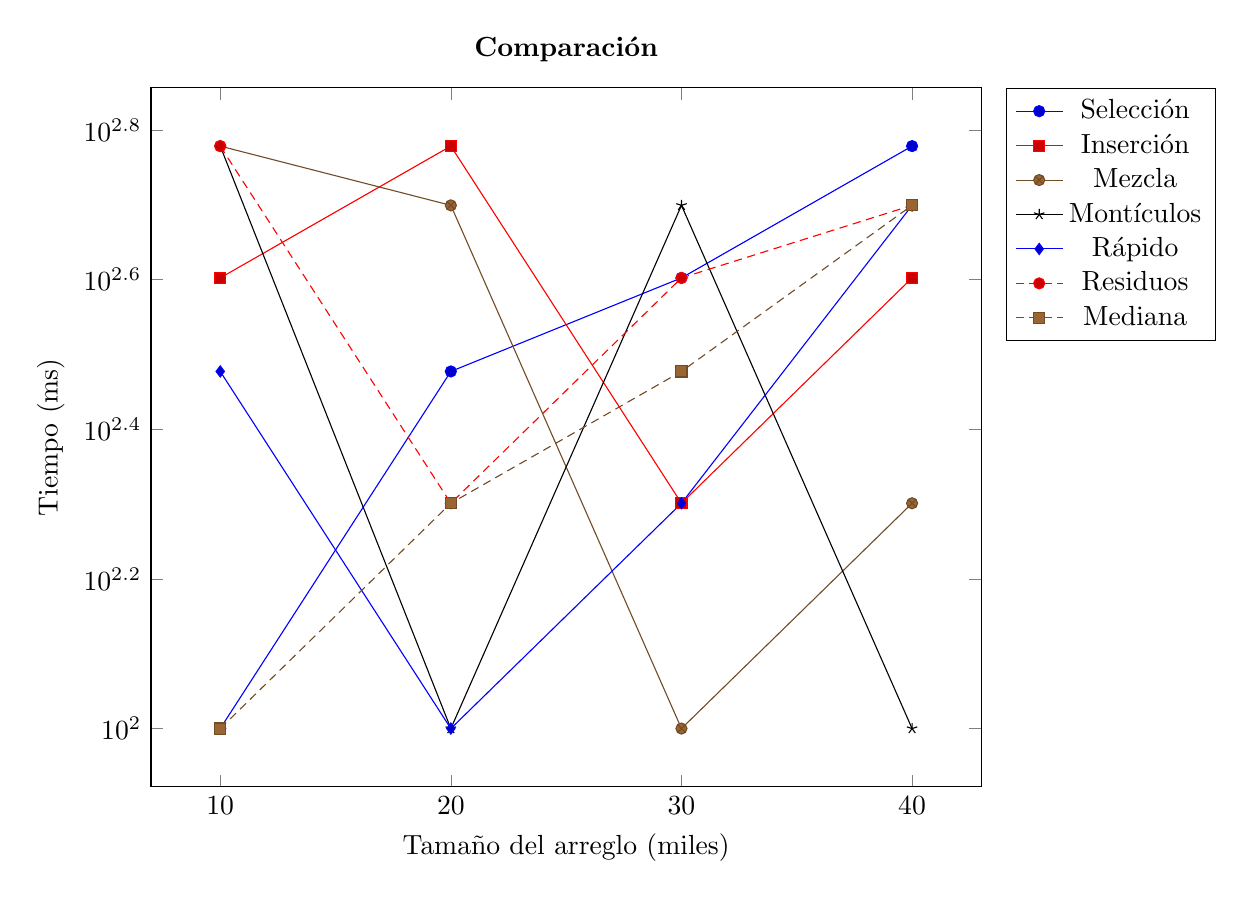
\begin{tikzpicture} 
    \begin{semilogyaxis}[
         width=\columnwidth,
         xtick={10,20,...,40},
         xlabel=Tamaño del arreglo (miles),
         ylabel=Tiempo (ms),
         legend pos=outer north east,
         title=\textbf{Comparación}]
    \addplot coordinates{(10,100) (20,300) (30,400) (40,600)};
    \addplot coordinates{(10,400) (20,600) (30,200) (40,400)};
    \addplot coordinates{(10,600) (20,500) (30,100) (40,200)};
    \addplot coordinates{(10,600) (20,100) (30,500) (40,100)};
    \addplot coordinates{(10,300) (20,100) (30,200) (40,500)};
    \addplot coordinates{(10,600) (20,200) (30,400) (40,500)};
    \addplot coordinates{(10,100) (20,200) (30,300) (40,500)};
    \legend{Selección,Inserción,Mezcla,Montículos,Rápido,Residuos,Mediana}
    \end{semilogyaxis}
\end{tikzpicture}
\par\end{centering}

\caption{Gráfico comparativo de los tiempos promedio de ejecución de los algoritmos.\label{fig:log}}
\end{figure*}
 Sin comentarios\ldots{} Lorem ipsum dolor sit amet, consetetur sadipscing
elitr, sed diam nonumy eirmod tempor invidunt ut labore et dolore
magna aliquyam erat, sed diam voluptua. At vero eos et accusam et
justo duo dolores et ea rebum. Stet clita kasd gubergren, no sea takimata
sanctus est Lorem ipsum dolor sit amet. Lorem ipsum dolor sit amet,
consetetur sadipscing elitr, sed diam nonumy eirmod tempor invidunt
ut labore et dolore magna aliquyam erat, sed diam voluptua.


\section{Conclusiones}

A partir de los resultados se concluye que\ldots{} Lorem ipsum
dolor sit amet, consetetur sadipscing elitr, sed diam nonumy eirmod
tempor invidunt ut labore et dolore magna aliquyam erat, sed diam
voluptua. At vero eos et accusam et justo duo dolores et ea rebum.
Stet clita kasd gubergren, no sea takimata sanctus est Lorem ipsum
dolor sit amet. Lorem ipsum dolor sit amet, consetetur sadipscing
elitr, sed diam nonumy eirmod tempor invidunt ut labore et dolore
magna aliquyam erat, sed diam voluptua.

Lorem ipsum dolor sit amet, consetetur sadipscing elitr, sed diam
nonumy eirmod tempor invidunt ut labore et dolore magna aliquyam erat,
sed diam voluptua. At vero eos et accusam et justo duo dolores et
ea rebum. Stet clita kasd gubergren, no sea takimata sanctus est Lorem
ipsum dolor sit amet. Lorem ipsum dolor sit amet, consetetur sadipscing
elitr, sed diam nonumy eirmod tempor invidunt ut labore et dolore
magna aliquyam erat, sed diam voluptua.


\appendices{}


\section{Código de los algoritmos}

El código se muestra en los algoritmos \ref{alg:saludo-tico} y \ref{alg:hello-world}.

\begin{algorithm}
\caption{Algoritmo que despliega en la salida estándar el saludo de los ticos.\label{alg:saludo-tico}}


\begin{lstlisting}[language={[ANSI]C++}]
int main() {
	cout << 'Pura vida!\n';
	return 0; 
}
\end{lstlisting}


\end{algorithm}
\begin{algorithm*}
\caption{Primer código que aprende un estudiante de programación. Si el código
no cabe en una columna, seleccione «extender columnas» en la configuración
del \emph{flotante} para que tome las dos columnas (como el flotante
de este algoritmo). En \protect\LaTeX{} use la versión «con estrella» del
entorno «algoritmo»: \texttt{\textbackslash{}begin\{algorithm{*}\}}
y \texttt{\textbackslash{}end\{algorithm{*}\}}. \label{alg:hello-world}}


\lstinputlisting[language={C++}]{Hello_world.cpp}
\end{algorithm*}


\bibliographystyle{IEEEtran}
\bibliography{Referencias}

\begin{IEEEbiography}[{\foreignlanguage{english}{%
\fbox{\begin{minipage}[t][1.25in]{1in}%
\selectlanguage{spanish}%
Replace this box by an image with a width of 1\,in and a height of
1.25\,in!\selectlanguage{english}%
%
\end{minipage}}}}]{Your Name}
 All about you and the what your interests are.\end{IEEEbiography}
 
 \begin{IEEEbiography}[{\foreignlanguage{english}{%
\fbox{\begin{minipage}[t][1.25in]{1in}%
\selectlanguage{spanish}%
Replace this box by an image with a width of 1\,in and a height of
1.25\,in!\selectlanguage{english}%
%
\end{minipage}}}}]{Your Name}
 All about you and the what your interests are.\end{IEEEbiography}



\end{document}
